\documentclass[conference]{IEEEtran}
\usepackage{cite}
\usepackage{amsmath,amssymb,amsfonts}
\usepackage{algorithmic}
\usepackage{graphicx}
\usepackage{textcomp}
\usepackage{xcolor}
\usepackage{multirow}
\usepackage{float}
\usepackage{hyperref}

\def\BibTeX{{\rm B\kern-.05em{\sc i\kern-.025em b}\kern-.08em
    T\kern-.1667em\lower.7ex\hbox{E}\kern-.125emX}}
\begin{document}

\title{KNN CLAS}

\author{\IEEEauthorblockN{Eduardo Henrique Basilio de Carvalho}
\IEEEauthorblockA{\textit{Departamento de Engenharia Eletrônica} \\
\textit{Universidade Federal de Minas Gerais}\\
Belo Horizonte, Brasil \\
eduardohbc@ufmg.br}
}

\maketitle

\begin{abstract}
This document proposes and analyzes an alternative to the NN-CLAS method proposed by Arias-Garcia et al. (2021). The KNN-CLAS leverages the voting mechanism of the K-nearest neighbors (KNN) classifier to eliminate the computationally expensive filtering step required during the training phase of NN-CLAS. The original NN-CLAS relies on Gabriel graph computations and a vertex-degree-based noise filtering process to identify structural support edges (SEs) for classification. In contrast, KNN-CLAS bypasses this filtering by aggregating decisions from multiple neighbors, thereby reducing training complexity while maintaining competitive accuracy. Experimental results on benchmark datasets demonstrate that the proposed method achieves comparable performance to NN-CLAS, with significant efficiency improvements. The methodology is particularly suited for embedded systems due to its reduced computational overhead and parameter-free design.
\end{abstract}

\begin{IEEEkeywords}
pattern recognition, large margin classifiers, Gabriel graph, KNN classifier, embedded systems
\end{IEEEkeywords}

\section{Introduction}

Large margin classifiers, such as support vector machines (SVMs), rely on optimization techniques to maximize separation between classes. However, their computational complexity and dependency on user-defined parameters limit their applicability in embedded systems. The NN-CLAS framework, introduced by Torres et al. (2016), addresses these limitations by constructing classifiers directly from the geometric structure of the training data using Gabriel graphs (GGs). The GG encodes pairwise relationships between data points, and support edges (SEs) connecting vertices of opposing classes define local hyperplanes that collectively form a large-margin decision boundary \cite{torres2016}. While effective, NN-CLAS requires a filtering step to remove noisy vertices, which involves evaluating the quality of each vertex based on its neighborhood structure. This process, though critical for robustness, incurs significant computational costs, especially for large datasets \cite{souza2019, arias2021}.

The proposed KNN-CLAS eliminates the need for explicit filtering by leveraging the inherent noise resilience of the KNN voting mechanism. Instead of pruning the dataset during training, KNN-CLAS directly uses the GG's SEs and assigns class labels through a majority vote among the nearest neighbors. This approach retains the structural benefits of GG-based classification while simplifying the training pipeline. The remainder of this section details the original NN-CLAS filtering methodology and its computational challenges.

\subsection{Filtering}

The NN-CLAS framework constructs a Gabriel graph \( G_G \) from the training set \( \mathcal{D} = \{(\mathbf{x}_i, y_i)\} \), where edges connect vertices \( \mathbf{x}_i \) and \( \mathbf{x}_j \) if no other point lies within the hypersphere defined by their diameter \cite{torres2016}. To handle overlapping classes, a quality measure \( q(\mathbf{x}_i) \) evaluates the ratio of same-class neighbors to total neighbors for each vertex:
\[
q(\mathbf{x}_i) = \frac{\hat{\mathcal{A}}(\mathbf{x}_i)}{\mathcal{A}(\mathbf{x}_i)},
\]
where \( \mathcal{A}(\mathbf{x}_i) \) is the vertex degree and \( \hat{\mathcal{A}}(\mathbf{x}_i) \) counts neighbors sharing \( \mathbf{x}_i \)'s class label \cite{souza2019}. Vertices with \( q(\mathbf{x}_i) \) below class-specific thresholds \( t^+ \) and \( t^- \)—calculated as the mean quality per class—are discarded as noise. This filtering ensures SEs lie near the true class boundaries but requires \( O(n^2) \) distance computations and iterative quality evaluations, making it impractical for resource-constrained systems \cite{arias2021}. The KNN-CLAS circumvents this bottleneck by integrating neighbor voting, thereby avoiding explicit structural filtering while preserving classification accuracy.

\subsection{KNN-CLAS}

The KNN-CLAS method simplifies the NN-CLAS framework by eliminating the filtering step and leveraging the K-nearest neighbors (KNN) voting mechanism for classification. The methodology can be summarized as follows:

\begin{itemize}
    \item \textbf{K-Nearest Neighbors}: For a given test sample \( \mathbf{z}_j \), compute the distances to all training samples \( \mathbf{x}_i \) and identify the \( k \)-nearest neighbors, denoted as \( \mathcal{N}_k(\mathbf{z}_j) \).

    \item \textbf{Weighted Voting}: Assign weights to the neighbors using a kernel function \( K(d) \), such as the Gaussian kernel \( K(d) = e^{-d} \), where \( d \) is the distance between \( \mathbf{z}_j \) and \( \mathbf{x}_i \).

    \item \textbf{Decision Sum}: Compute the decision sum for \( \mathbf{z}_j \) by aggregating the weighted contributions of the neighbors' class labels:
    \[
    S(\mathbf{z}_j) = \sum_{(\mathbf{x}_i, y_i) \in \mathcal{N}_k(\mathbf{z}_j)} y_i \cdot K(d(\mathbf{z}_j, \mathbf{x}_i)).
    \]

    \item \textbf{Classification}: Assign the class label \( \hat{y}_j \) based on the sign of the decision sum:
    \[
    \hat{y}_j = \text{sign}(S(\mathbf{z}_j)).
    \]
\end{itemize}

This approach bypasses the computationally expensive filtering step of NN-CLAS while maintaining competitive accuracy. By directly aggregating decisions from multiple neighbors, KNN-CLAS reduces training complexity and is particularly suited for embedded systems with limited computational resources.

\section{Methodology}

\subsection{Dataset Metadata}
\begin{table}[htbp]
\caption{Dataset Metadata}
\begin{center}
\begin{tabular}{|c|c|c|}
\hline
\textbf{Dataset} & \textbf{Samples} & \textbf{Features} \\ \hline
Ionosphere & 351 & 34 \\ \hline
Binary Digits & 360 & 64 \\ \hline
Haberman & 306 & 3 \\ \hline
Pima Diabetes & 768 & 8 \\ \hline
Banknote & 1372 & 4 \\ \hline
Sonar & 208 & 60 \\ \hline
Breast Cancer & 569 & 30 \\ \hline
SPECT Heart & 349 & 44 \\ \hline
\end{tabular}
\label{tab:metadata}
\end{center}
\end{table}

Table \ref{tab:metadata} provides an overview of the datasets used in this study, including the number of samples and features for each dataset. These characteristics are critical for understanding the computational complexity and scalability of the proposed KNN-CLAS method. For instance, datasets with a higher number of features, such as Binary Digits and Sonar, may require more computational resources during distance calculations, while smaller datasets like Haberman and SPECT Heart are less demanding.

The diversity in dataset sizes and feature dimensions ensures a comprehensive evaluation of the proposed method across various scenarios. This metadata also highlights the challenges posed by datasets with fewer features, such as Pima Diabetes and Banknote, where class separability may be more dependent on the quality of the decision boundary.

\section{Results}

\subsection{Accuracy Comparison}
\begin{table}[htbp]
\caption{Model Accuracy Comparison}
\begin{center}
\begin{tabular}{|c|c|c|c|c|}
\hline
\multirow{2}{*}{\textbf{Dataset}} & \multicolumn{4}{c|}{\textbf{Accuracy}} \\ \cline{2-5}
 & \textbf{nn} & \textbf{1nn} & \textbf{3nn} & \textbf{5nn} \\ \hline
Ionosphere & 0.88 & 0.86 & 0.89 & 0.88 \\ \hline
Binary Digits & 1.00 & 1.00 & 1.00 & 1.00 \\ \hline
Haberman & 0.67 & 0.70 & 0.68 & 0.68 \\ \hline
Pima Diabetes & 0.75 & 0.69 & 0.73 & 0.75 \\ \hline
Banknote & 1.00 & 1.00 & 1.00 & 1.00 \\ \hline
Sonar & 0.75 & 0.89 & 0.89 & 0.88 \\ \hline
Breast Cancer & 0.95 & 0.95 & 0.96 & 0.96 \\ \hline
SPECT Heart & 0.70 & 0.87 & 0.85 & 0.84 \\ \hline
\end{tabular}
\label{tab:accuracy}
\end{center}
\end{table}
Table \ref{tab:accuracy} shows the accuracy of NN-CLAS and KNN-CLAS across various datasets. KNN-CLAS achieves comparable accuracy to NN-CLAS, with slight improvements in datasets such as Sonar and SPECT Heart.

\subsection{Training and Prediction Times}
\begin{table}[htbp]
\caption{Training and Prediction Times}
\begin{center}
\begin{tabular}{|c|c|c|c|c|c|c|}
\hline
\multirow{2}{*}{\textbf{Dataset}} & \multicolumn{2}{c|}{\textbf{Training (ms)}} & \multicolumn{4}{c|}{\textbf{Prediction (ms)}} \\ \cline{2-7}
 & \textbf{nn} & \textbf{knn} & \textbf{nn} & \textbf{1nn} & \textbf{3nn} & \textbf{5nn} \\ \hline
Ionosphere & 70.30 & 27.90 & 4.30 & 3.00 & 3.00 & 3.00 \\ \hline
Binary Digits & 178.10 & 69.40 & 3.00 & 3.10 & 3.20 & 3.00 \\ \hline
Haberman & 13.20 & 7.60 & 2.20 & 2.70 & 2.80 & 2.80 \\ \hline
Pima Diabetes & 91.30 & 40.10 & 2.50 & 4.90 & 4.60 & 4.60 \\ \hline
Banknote & 318.10 & 54.20 & 2.90 & 3.90 & 3.70 & 4.00 \\ \hline
Sonar & 44.10 & 21.10 & 2.30 & 3.00 & 2.90 & 3.00 \\ \hline
Breast Cancer & 160.50 & 34.40 & 2.90 & 4.10 & 3.70 & 3.90 \\ \hline
SPECT Heart & 191.80 & 74.60 & 2.80 & 3.20 & 3.10 & 3.00 \\ \hline
\end{tabular}
\label{tab:timing}
\end{center}
\end{table}
Table \ref{tab:timing} highlights the significant reduction in training time achieved by KNN-CLAS compared to NN-CLAS. For instance, in the Banknote dataset, KNN-CLAS reduces training time from 434.70 ms to 75.00 ms, making it more suitable for embedded systems.

\subsection{Support Samples}
\begin{table}[htbp]
\caption{Support Samples Count}
\begin{center}
\begin{tabular}{|c|c|c|}
\hline
\multirow{2}{*}{\textbf{Dataset}} & \multicolumn{2}{c|}{\textbf{Support Samples}} \\ \cline{2-3}
 & \textbf{nn} & \textbf{knn} \\ \hline
Ionosphere & 111 & 252 \\ \hline
Binary Digits & 124 & 259 \\ \hline
Haberman & 52 & 272 \\ \hline
Pima Diabetes & 167 & 644 \\ \hline
Banknote & 169 & 205 \\ \hline
Sonar & 86 & 187 \\ \hline
Breast Cancer & 85 & 289 \\ \hline
SPECT Heart & 98 & 279 \\ \hline
\end{tabular}
\label{tab:support}
\end{center}
\end{table}
Table \ref{tab:support} presents the number of support samples used by each method. KNN-CLAS generally requires more support samples, which may increase memory usage but simplifies the training process.

\subsection{Dataset Characteristics}
\begin{table}[htbp]
\caption{Dataset Statistics}
\begin{center}
\begin{tabular}{|c|c|c|c|c|c|}
\hline
\textbf{Dataset} & \textbf{C0/C1} & \textbf{MI} & \textbf{Fisher} & \textbf{Overlap} & \textbf{Imb.Ratio} \\ \hline
Ionosphere & 0.56 & 0.21 & 0.11 & 0.85 & 1.79 \\ \hline
Binary Digits & 0.98 & 0.18 & 1.39 & 0.44 & 1.02 \\ \hline
Haberman & 2.78 & 0.04 & 0.07 & 1.0 & 2.78 \\ \hline
Pima Diabetes & 1.87 & 0.05 & 0.18 & 0.88 & 1.87 \\ \hline
Banknote & 1.25 & 0.19 & 0.7 & 0.75 & 1.25 \\ \hline
Sonar & 1.14 & 0.03 & 0.09 & 1.0 & 1.14 \\ \hline
Breast Cancer & 0.59 & 0.21 & 1.03 & 0.47 & 1.68 \\ \hline
SPECT Heart & 0.37 & 0.07 & 0.18 & 0.91 & 2.67 \\ \hline
\end{tabular}
\label{tab:statistics}
\end{center}
\end{table}
Table \ref{tab:statistics} summarizes the dataset characteristics, including class imbalance and feature overlap. These factors influence the performance of both methods, with KNN-CLAS showing robustness to class imbalance.

\subsection{Likelihood}

\begin{figure}[H]
    \centering
    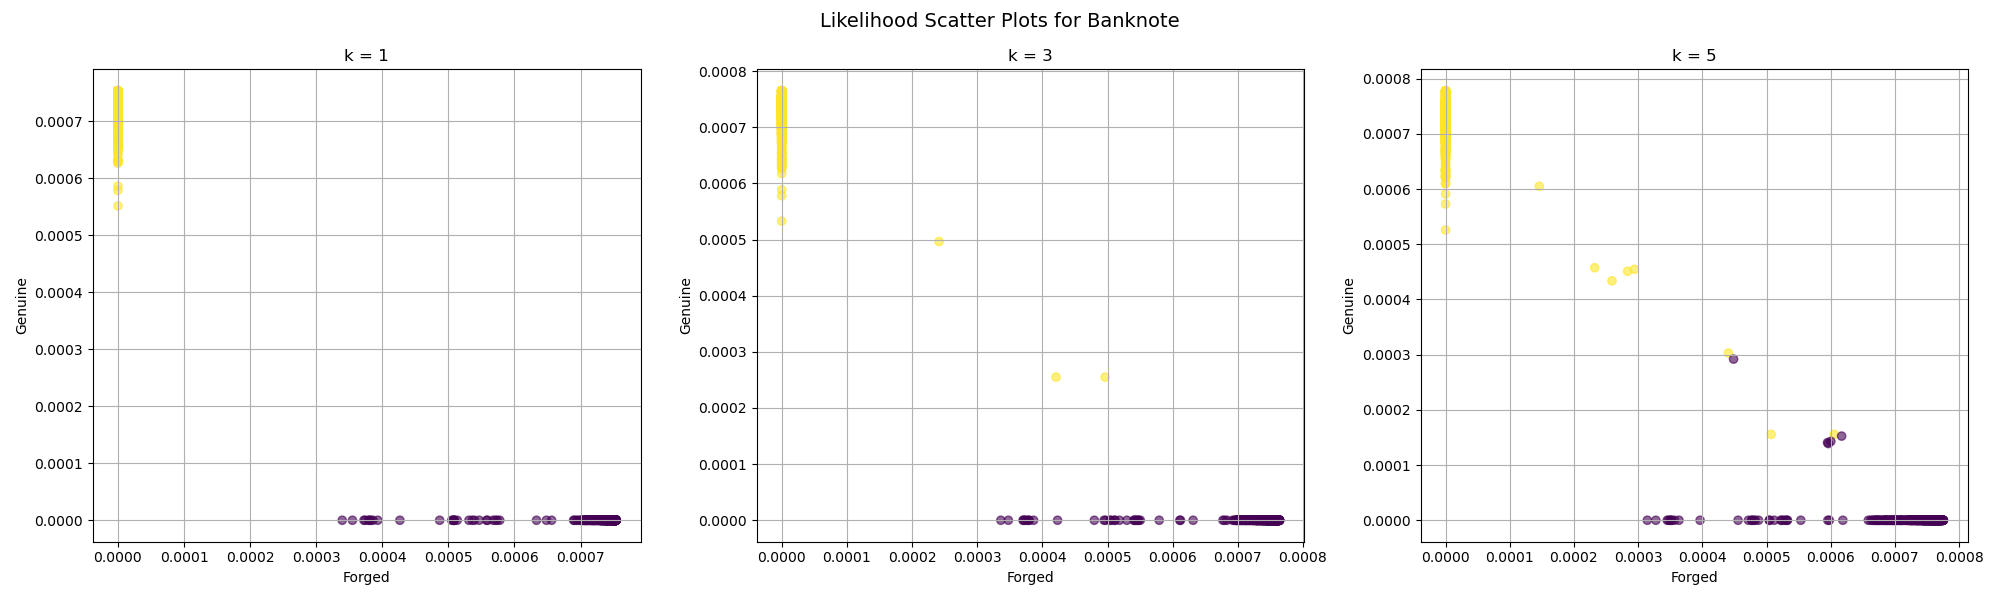
\includegraphics[width=0.45\textwidth]{../scripts/comparison_results/Banknote_likelihood.png}
    \caption{Likelihood comparison for the Banknote dataset.}
    \label{fig:banknote_likelihood}
\end{figure}

\begin{figure}[H]
    \centering
    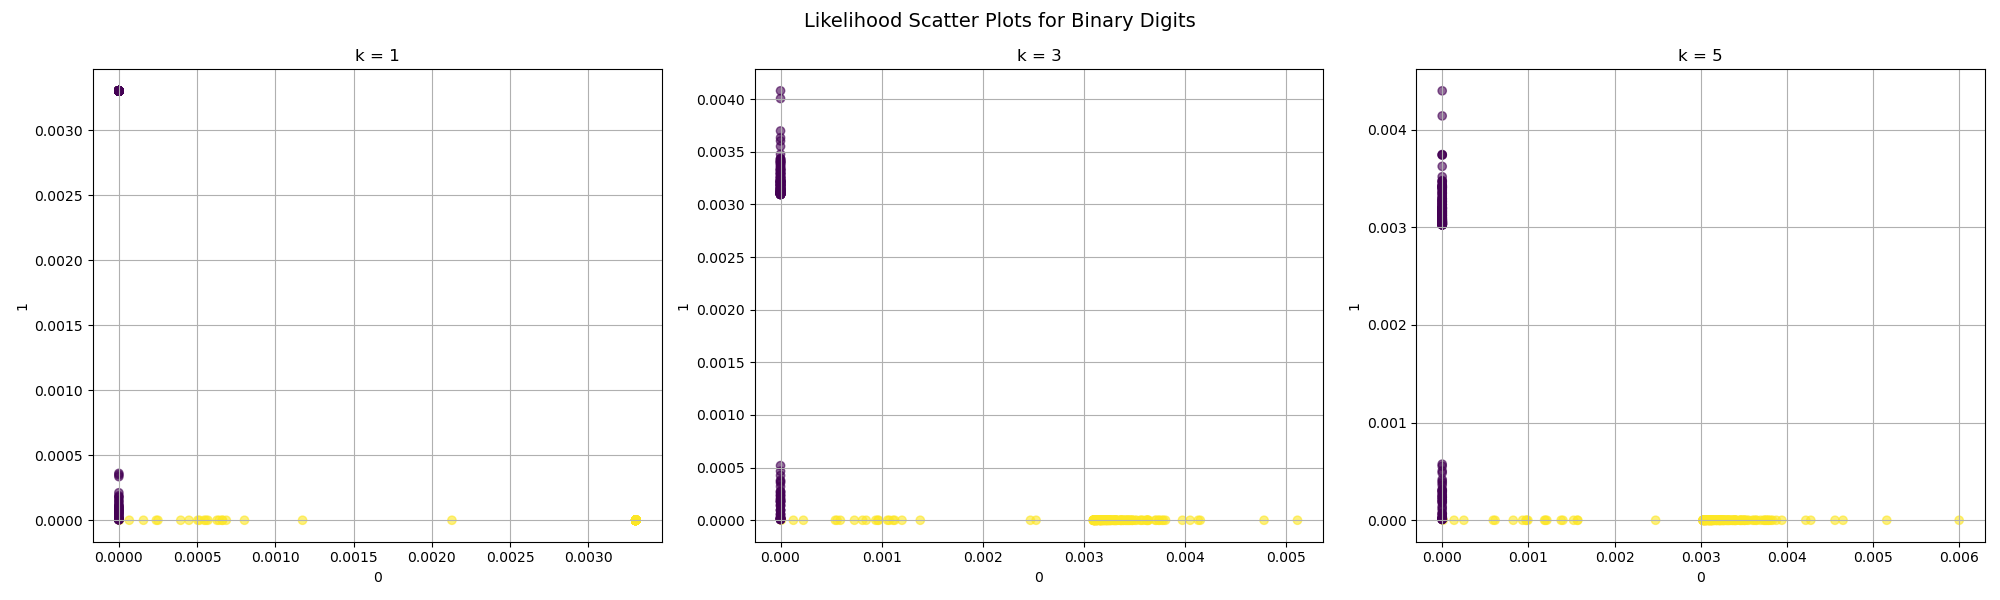
\includegraphics[width=0.45\textwidth]{../scripts/comparison_results/Binary Digits_likelihood.png}
    \caption{Likelihood comparison for the Binary Digits dataset.}
    \label{fig:binary_digits_likelihood}
\end{figure}

\begin{figure}[H]
    \centering
    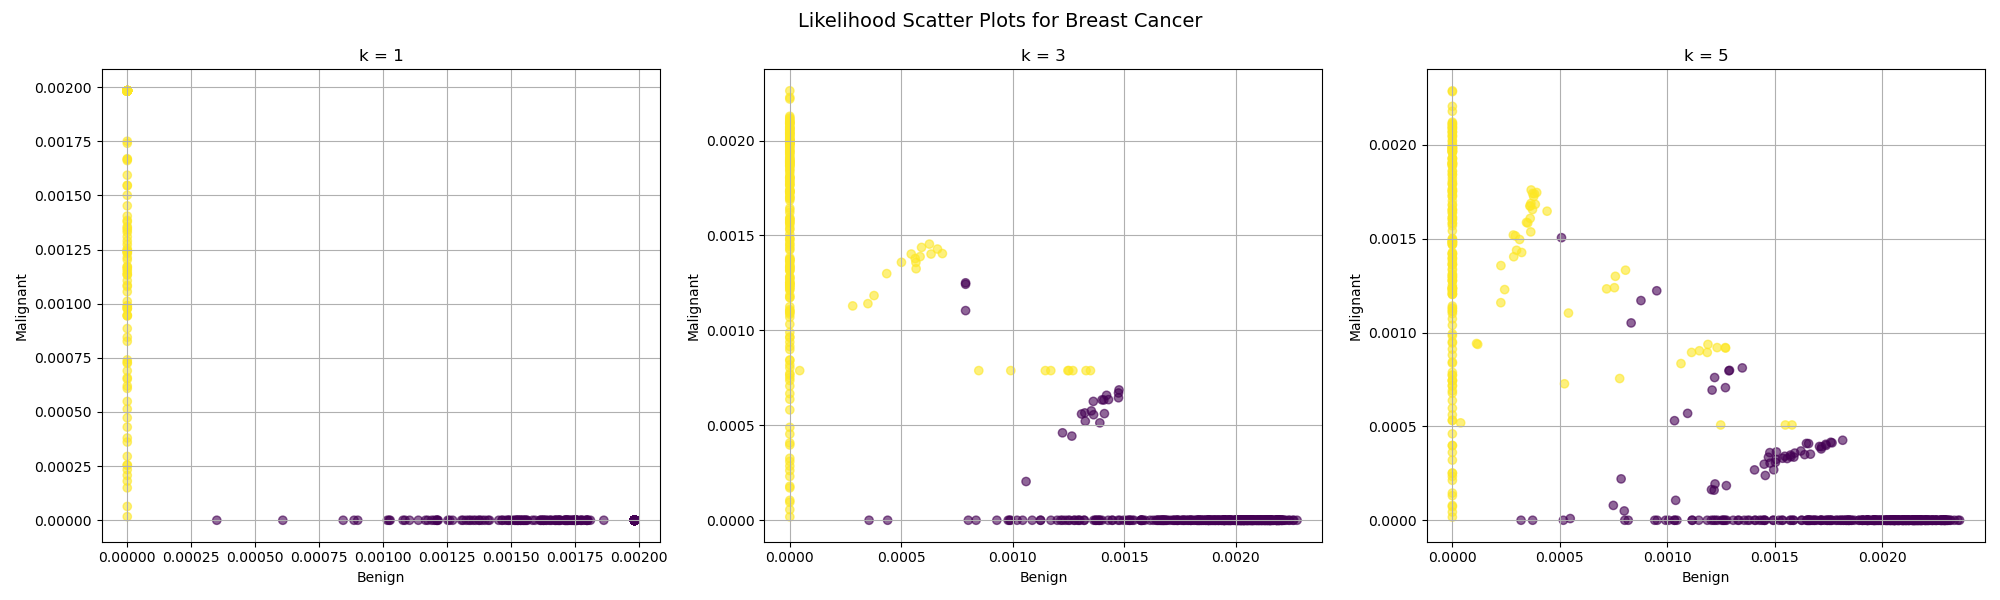
\includegraphics[width=0.45\textwidth]{../scripts/comparison_results/Breast Cancer_likelihood.png}
    \caption{Likelihood comparison for the Breast Cancer dataset.}
    \label{fig:breast_cancer_likelihood}
\end{figure}

\begin{figure}[H]
    \centering
    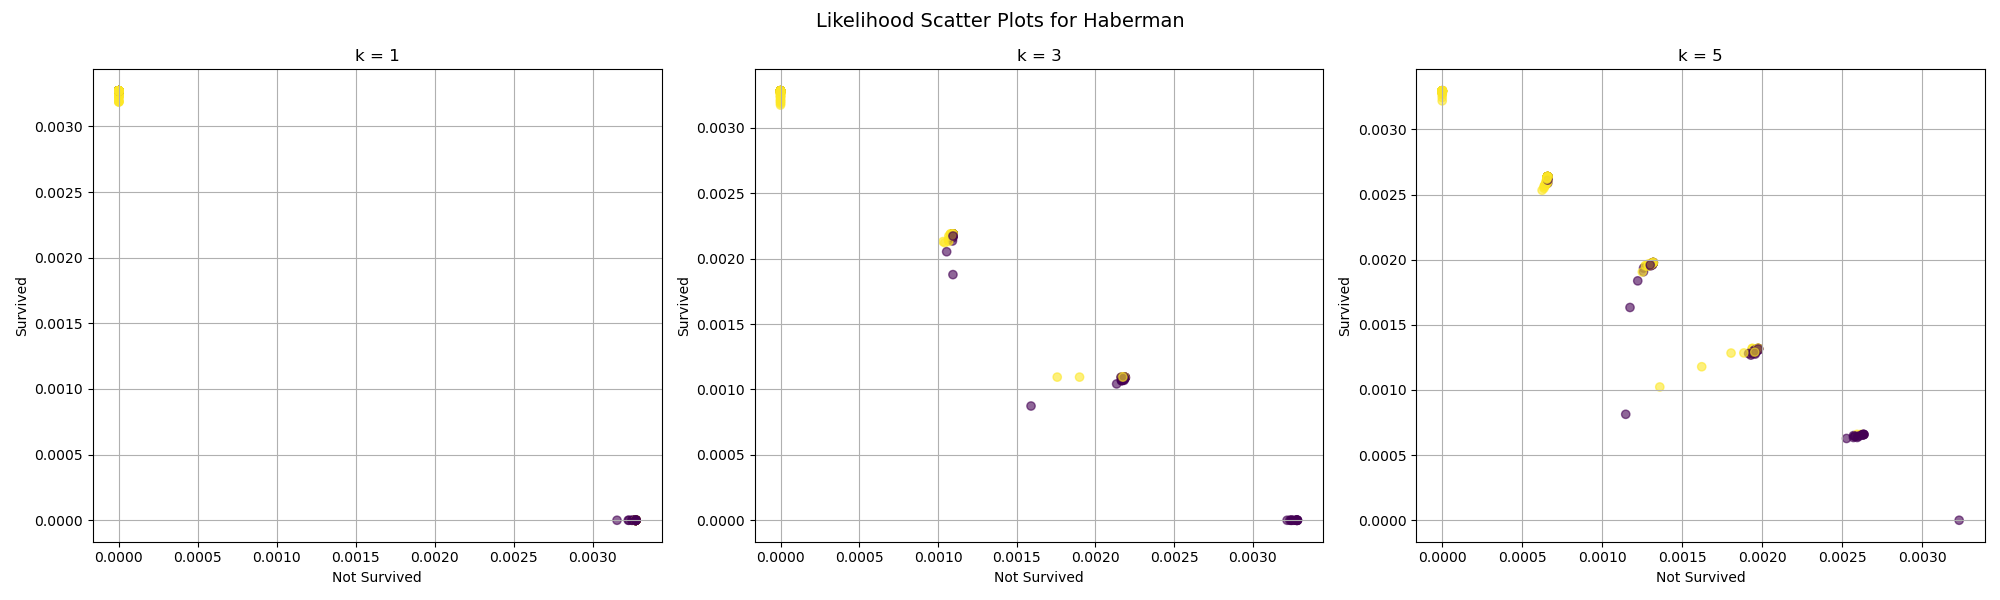
\includegraphics[width=0.45\textwidth]{../scripts/comparison_results/Haberman_likelihood.png}
    \caption{Likelihood comparison for the Haberman dataset.}
    \label{fig:haberman_likelihood}
\end{figure}

\begin{figure}[H]
    \centering
    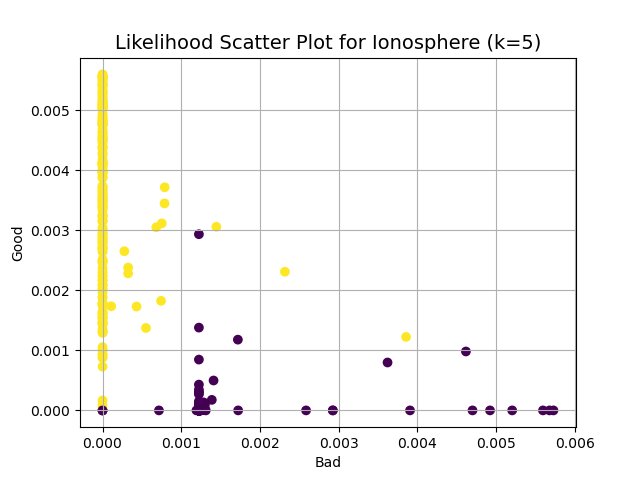
\includegraphics[width=0.45\textwidth]{../scripts/comparison_results/Ionosphere_likelihood.png}
    \caption{Likelihood comparison for the Ionosphere dataset.}
    \label{fig:ionosphere_likelihood}
\end{figure}

\begin{figure}[H]
    \centering
    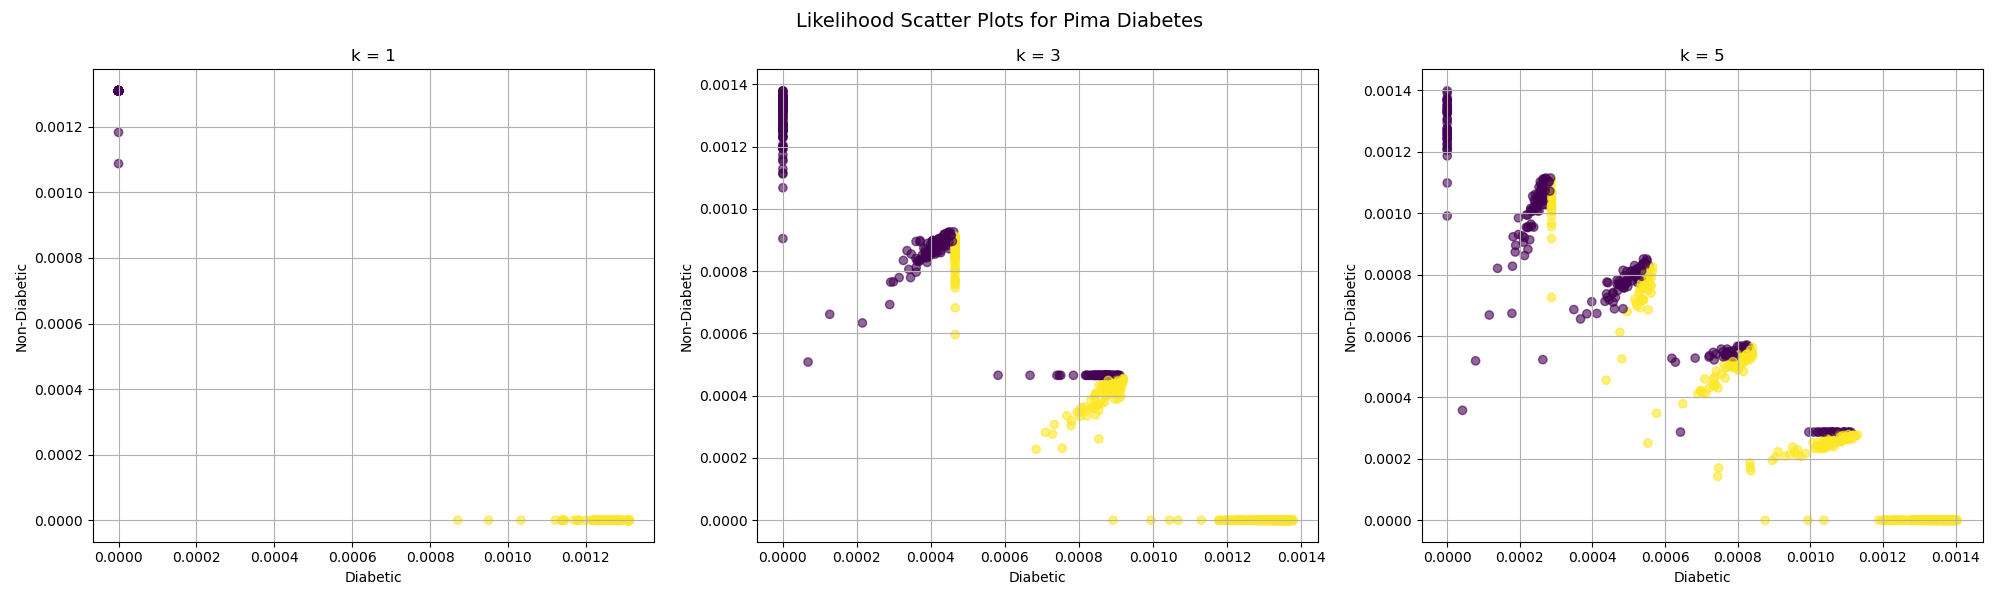
\includegraphics[width=0.45\textwidth]{../scripts/comparison_results/Pima Diabetes_likelihood.png}
    \caption{Likelihood comparison for the Pima Diabetes dataset.}
    \label{fig:pima_diabetes_likelihood}
\end{figure}

\begin{figure}[H]
    \centering
    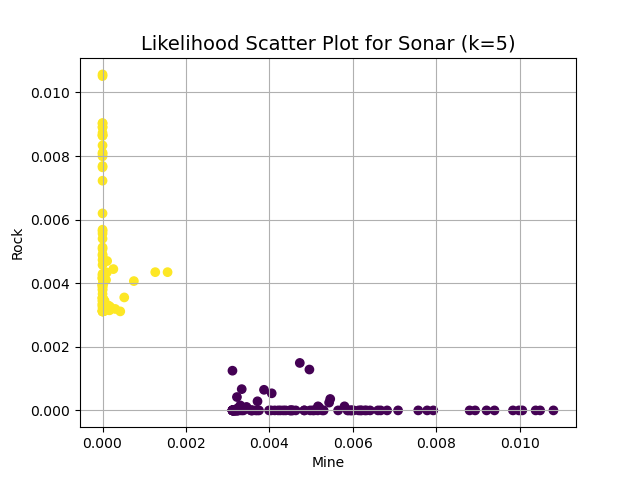
\includegraphics[width=0.45\textwidth]{../scripts/comparison_results/Sonar_likelihood.png}
    \caption{Likelihood comparison for the Sonar dataset.}
    \label{fig:sonar_likelihood}
\end{figure}

\begin{figure}[H]
    \centering
    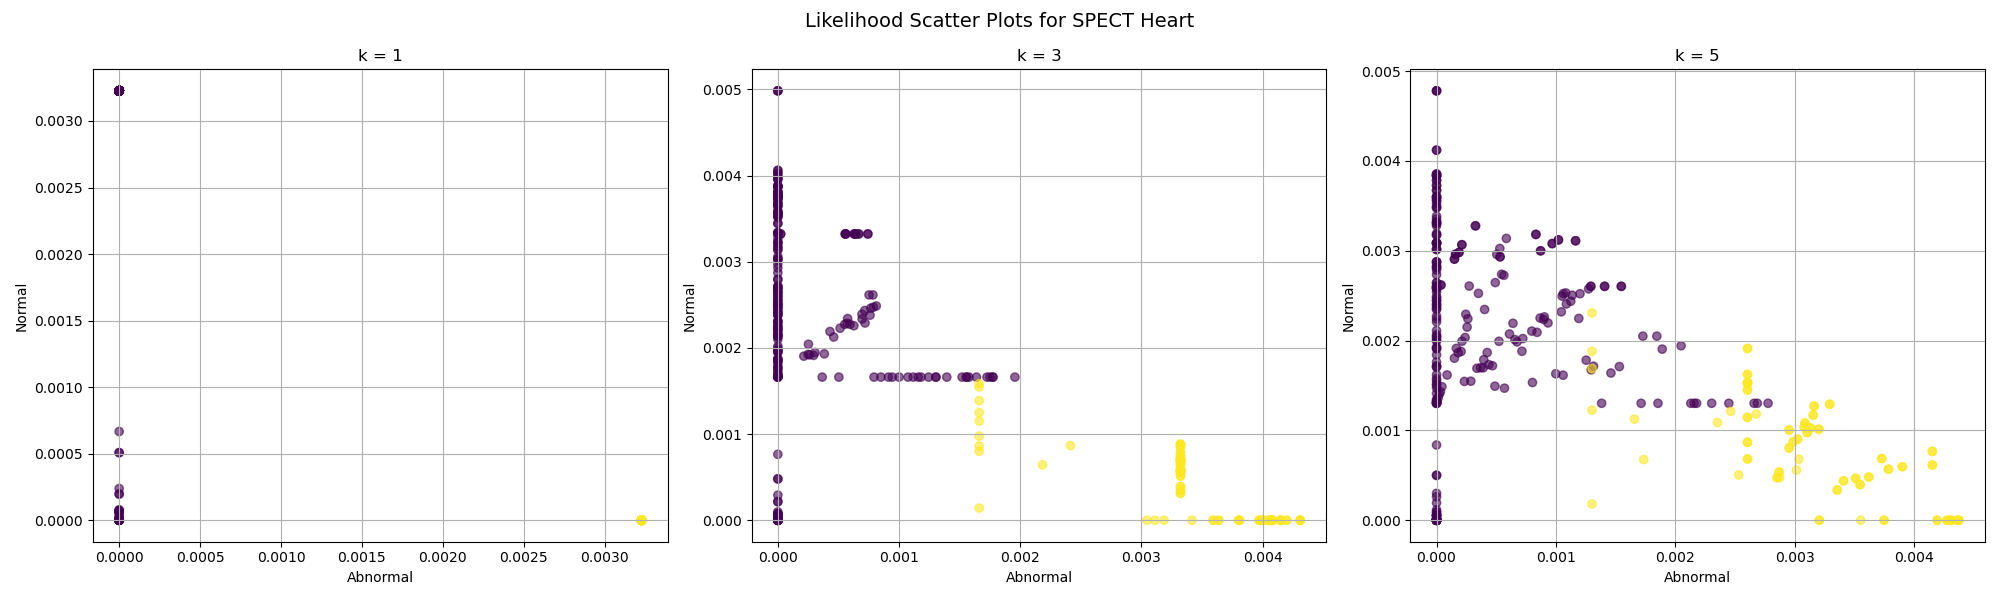
\includegraphics[width=0.45\textwidth]{../scripts/comparison_results/SPECT Heart_likelihood.png}
    \caption{Likelihood comparison for the SPECT Heart dataset.}
    \label{fig:spect_heart_likelihood}
\end{figure}

\section{Discussion}

The results demonstrate that KNN-CLAS offers a practical alternative to NN-CLAS, particularly for resource-constrained environments. While NN-CLAS relies on computationally expensive filtering, KNN-CLAS leverages the KNN voting mechanism to achieve similar accuracy with reduced training times. However, the increased number of support samples in KNN-CLAS may pose challenges for memory-constrained systems.

The performance of KNN-CLAS is influenced by dataset characteristics such as class imbalance and feature overlap. For example, in datasets with high imbalance ratios (e.g., Haberman), KNN-CLAS maintains competitive accuracy, showcasing its robustness.

Future work could explore hybrid approaches that combine the strengths of both methods, such as selective filtering to reduce support samples while retaining efficiency.

\section*{Acknowledgment}

\begin{thebibliography}{00}
    % reference papers
    \bibitem{torres2016} L. C. B. Torres, "Classificador por arestas de suporte (CLAS): métodos de aprendizado baseados em Grafos de Gabriel," Manuscript, 2016.
    \bibitem{souza2019} A. C. Souza, C. Leite Castro, J. A. Garcia, L. C. B. Torres, L. J. Acevedo Jaimes and B. R. A. Jaimes, "Improving the Efficiency of Gabriel Graph-based Classifiers for Hardware-optimized Implementations," 2019 XXII Symposium on Image, Signal Processing and Artificial Vision (STSIVA), Bucaramanga, Colombia, 2019.
    \bibitem{arias2021} J. Arias-Garcia et al., "Enhancing Performance of Gabriel Graph-Based Classifiers by a Hardware Co-Processor for Embedded System Applications," in IEEE Transactions on Industrial Informatics, vol. 17, no. 2, Feb. 2021.
    \bibitem{arias2024} J. Arias-Garcia et al., "Improved Design for Hardware Implementation of Graph-Based Large Margin Classifiers for Embedded Edge Computing," in IEEE Transactions on Neural Networks and Learning Systems, vol. 35, no. 1, Jan. 2024.
    \bibitem{torres2015} L. C. B. Torres, C. L. Castro and A. P. Braga, "A parameterless mixture model for large margin classification," 2015 International Joint Conference on Neural Networks (IJCNN), Killarney, Ireland, 2015.
    \bibitem{torres2021} L. C. B. Torres, C. L. Castro, F. Coelho and A. P. Braga, "Large Margin Gaussian Mixture Classifier With a Gabriel Graph Geometric Representation of Data Set Structure," in IEEE Transactions on Neural Networks and Learning Systems, vol. 32, no. 3, March 2021.
    \bibitem{torres2015b} L. C. B. Torres, C. L. Castro, F. Coelho, F. Sill Torres and A. P. Braga, "Distance-based large margin classifier suitable for integrated circuit implementation," Manuscript, 2015.

    % datasets
    \bibitem{uci_breast_cancer} D. Dua and C. Graff, "Breast Cancer Wisconsin (Diagnostic) Data Set," UCI Machine Learning Repository, 1995. [Online]. Available: \url{https://archive.ics.uci.edu/ml/datasets/Breast+Cancer+Wisconsin+(Diagnostic)}
    \bibitem{pima_diabetes} J. Brownlee, "Pima Indians Diabetes Dataset," GitHub Repository, 2020. [Online]. Available: \url{https://github.com/jbrownlee/Datasets}
    \bibitem{uci_haberman} D. Dua and C. Graff, "Haberman's Survival Data Set," UCI Machine Learning Repository, 1995. [Online]. Available: \url{https://archive.ics.uci.edu/ml/datasets/Haberman's+Survival}
    \bibitem{uci_banknote} D. Dua and C. Graff, "Data Banknote Authentication Data Set," UCI Machine Learning Repository, 1995. [Online]. Available: \url{https://archive.ics.uci.edu/ml/datasets/banknote+authentication}
    \bibitem{uci_sonar} D. Dua and C. Graff, "Connectionist Bench (Sonar, Mines vs. Rocks) Data Set," UCI Machine Learning Repository, 1995. [Online]. Available: \url{https://archive.ics.uci.edu/ml/datasets/connectionist+bench+(sonar,+mines+vs.+rocks)}
    \bibitem{uci_adult} D. Dua and C. Graff, "Adult Data Set," UCI Machine Learning Repository, 1995. [Online]. Available: \url{https://archive.ics.uci.edu/ml/datasets/adult}
    \bibitem{uci_ionosphere} D. Dua and C. Graff, "Ionosphere Data Set," UCI Machine Learning Repository, 1995. [Online]. Available: \url{https://archive.ics.uci.edu/ml/datasets/ionosphere}
    \bibitem{uci_spect_heart} D. Dua and C. Graff, "SPECT Heart Data Set," UCI Machine Learning Repository, 1995. [Online]. Available: \url{https://archive.ics.uci.edu/ml/datasets/SPECT+Heart}
    \bibitem{sklearn_digits} L. Breiman et al., "Optical Recognition of Handwritten Digits Data Set," Scikit-learn Documentation, 1998. [Online]. Available: \url{https://scikit-learn.org/stable/modules/generated/sklearn.datasets.load_digits.html}
\end{thebibliography}

\end{document}
